\setcounter{chapter}{-1}
\notocchapter{Prologue}

\sidefigure{AI art generated by VQGAN + CLIP \citep{esser_taming_2021,radford_learning_2021}. Prompt: \emph{\enquote{a huge ocean wave unsplash}}.}[fig:vqgan-1]{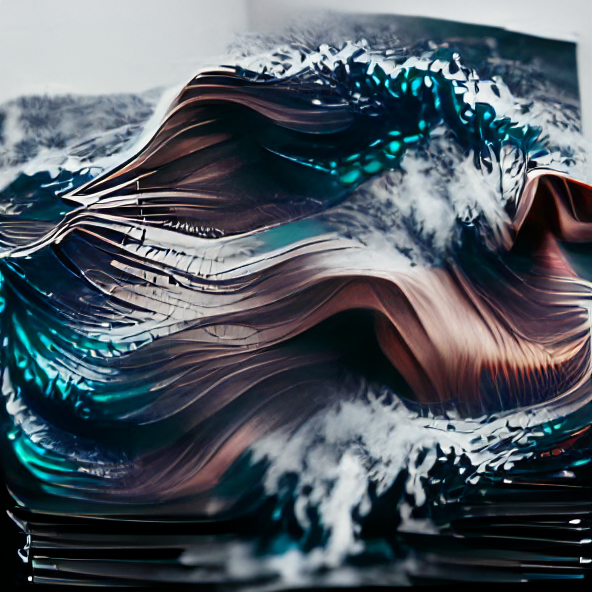
\includegraphics[width=.9\linewidth]{vqgan-images/vqgan-48}}
%
This PhD thesis is about the combination of rogue waves and machine learning. And what a combination that is! One is an unexpected menace, preying on anyone brave or stupid enough to enter its domain, with the sole purpose of pulling them into the abyss. The other is an unusually big wave in the ocean.

Machine learning, and especially deep learning, has rapidly transformed the world. Since the first large-scale applications of artificial neural networks in the early 2010's we have seen unparalleled machine performance in natural language processing \citep{gpt3,bert}, image recognition \citep{alexnet}, recommender systems \citep{ma2020temporal}, generative art \citep[\figref{fig:vqgan-1};][]{esser_taming_2021}, chess \citep{silver_mastering_2017}, Go \citep{silver_mastering_2016}, and StarCraft II \citep{vinyals_grandmaster_2019}. Entire industries have been transformed, to the point that previously \enquote{analogue} companies like Walmart and Home Depot are now publishing machine learning research \citep[\eg][]{xu_self-attention_2019,homedepot}.

And yet, despite almost unprecedented levels of enthusiasm in its adoption (and funding), it is still surprisingly difficult to use machine learning to answer scientific questions.

In fact, there are few examples where machine learning has directly led to scientific \emph{discovery} \citep{succi_big_2019}. That is in part because the goals of machine learning --- at least the kind that has led to the successes described above --- are often opposed to the goals of science. Science is about finding universal laws that encapsulate a causal relationship in our world so that we understand it better. Machine learning on the other hand performs best when \enquote{good enough} is an acceptable outcome, and where it doesn't matter how the algorithm arrives at its answer. This disconnect has not gone unnoticed in machine learning research \citep{marcus_deep_2022}, especially since some areas where machine learning \emph{should} do well \citep[like driverless cars or medical diagnoses,][]{varoquaux2021failed} prove so far elusive.

One promising line of research to address this is causality, where statistical models are imbued with the capability to perform causal reasoning \citep[see \eg][]{runge_inferring_2019}. This allows algorithms to uncover causal connections instead of associations (causal discovery), especially if we allow agents to suggest experiments (interventions) and observe the outcome. But we are still a long way from large-scale adoption of these tools.

In the meantime, the goal of this PhD thesis is to explore how we can use machine learning \emph{today} to understand a real physical phenomenon. Because ultimately, despite their issues, machine learning models are immensely powerful products of mathematics and engineering capable of large-scale data processing like no other. In this study we use machine learning mostly as a tool for large-scale data analysis and inference, prioritizing understanding (and discovery) over prediction. This turns out to be a powerful approach\sidenote[-0.6]{\citet{voit_perspective_2019} calls this \enquote{data mining-based induction} and even postulates this to become a fundamental extension to the scienfic method.}, but also a very challenging one that is inherently interdisciplinary and requires a solid foundation in both machine learning and the target scientific domain.

Rogue waves as a study object do not make this task any easier. Most machine learning algorithms struggle with low probabilities, and in the case of rogue waves, they are excessively low. But on the other hand, this also makes them a good target to study with machine learning: Low probabilities imply the need to process massive amounts of data that are difficult to analyze with traditional methods (let alone with human intuition). And of course, they are a fascinating phenomenon that I am proud to have been working on for the past 3 years.
